% Generated by `python -m experiments.experiment_1.appendix_captions` -- do not edit by hand.
% Main-text figure for Experiment 1. Needs \usepackage{graphicx,amsmath,amssymb};
% paths are relative to outputs/finals/experiment-1/.
\begin{figure}[tbp]
  \centering
  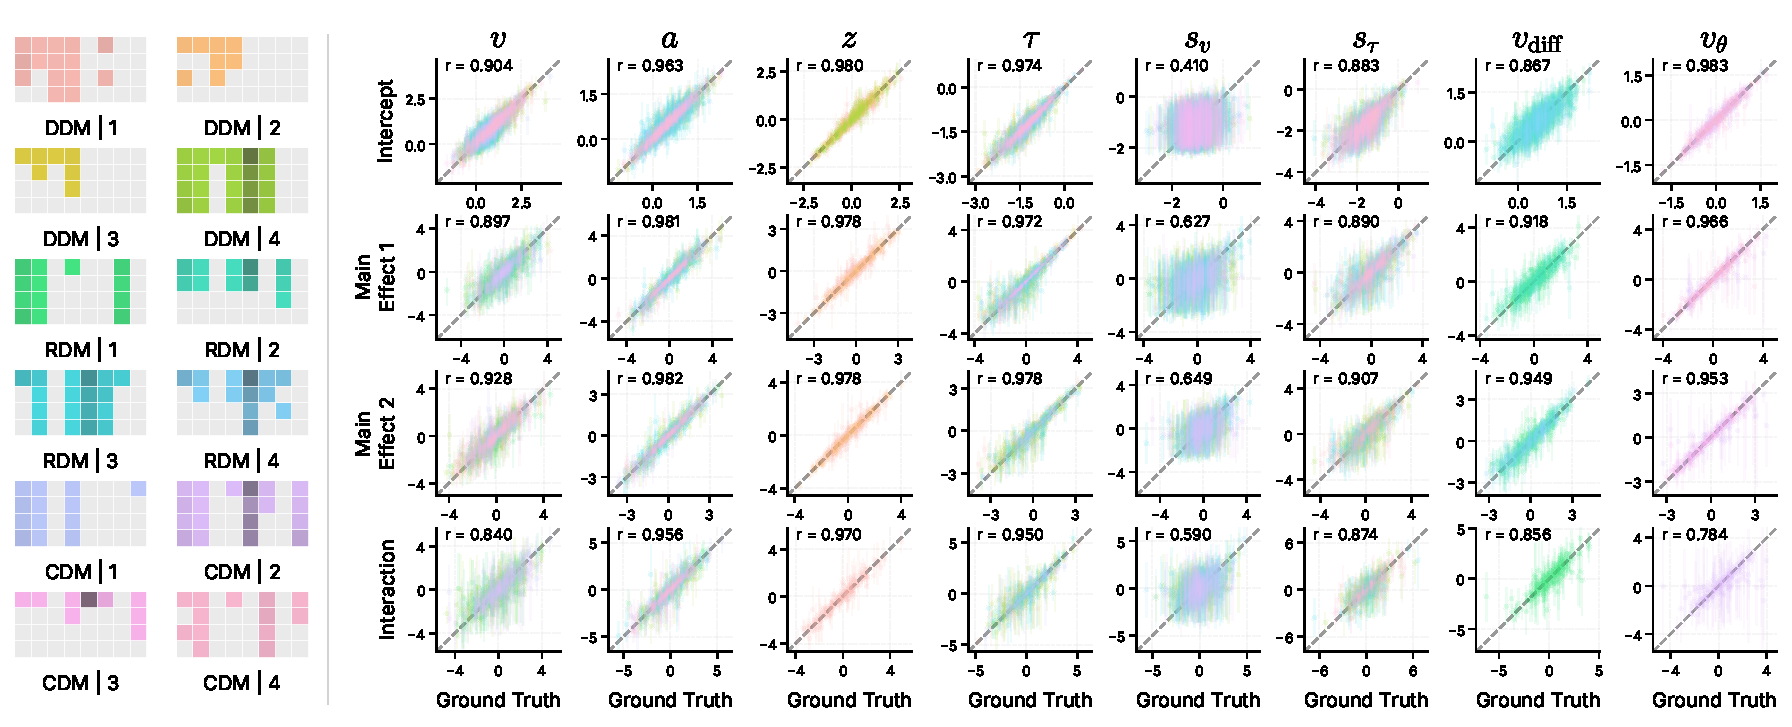
\includegraphics[width=\textwidth]{random_ensemble/recovery.pdf}\par\vspace{1ex}
  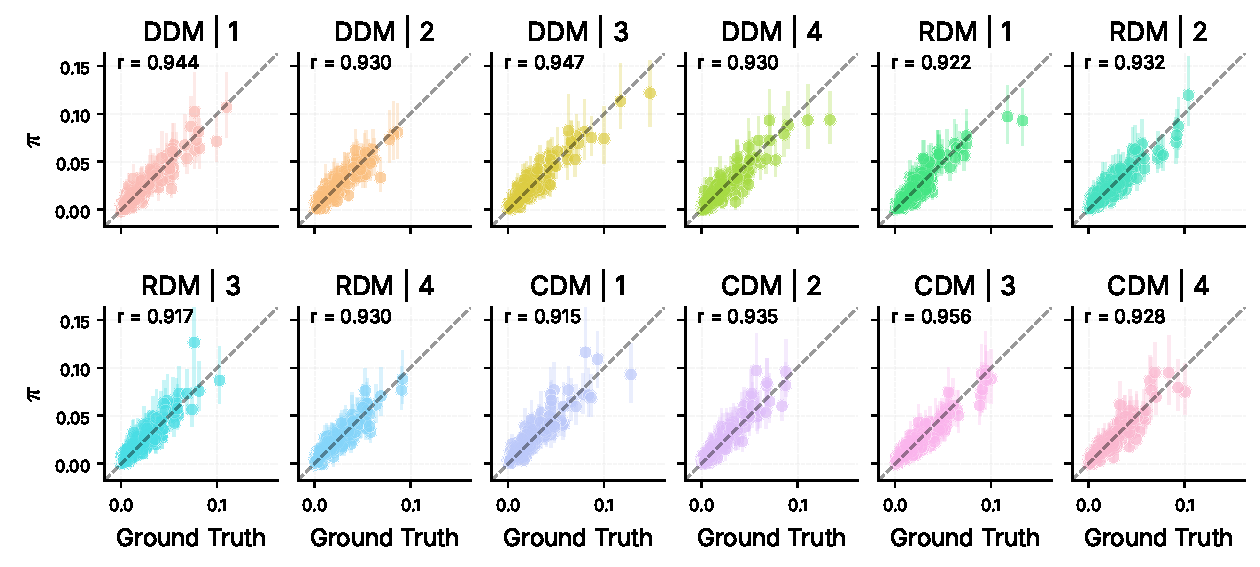
\includegraphics[width=0.85\textwidth]{random_ensemble/recovery_pi.pdf}\par\vspace{1ex}
  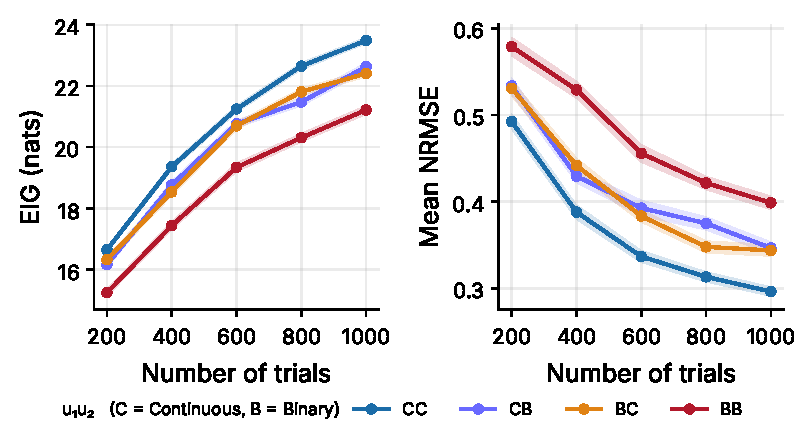
\includegraphics[width=0.75\textwidth]{information_gain/information_gain.pdf}
  \caption{\textbf{Amortized inference across design space.} Top: parameter recovery for 12 randomly drawn regression designs (4 per model family; two continuous or binary regressors and their interaction), all estimated by one CogFormer network: posterior means against ground truth with 90\% credible intervals, one colour per design; $r$ is the mean per-design correlation. Columns are the parameters of all three families and rows the coefficients (intercept, main effects of $u_1$ and $u_2$, interaction); the strip on the left shows each design's coefficient pattern, with opacity proportional to its $|r|$. Middle: the contamination probability $\pi$ for each design. Bottom: expected information gain (left) and mean NRMSE (right) against trial count when each of two DDM predictors is measured continuously (C) or as a binary factor (B); bands are $\pm 1$ standard error. Every estimate is an amortized forward pass of the same network. Details in Appendix~\ref{app:exp1-main-details}.}
  \label{fig:exp1-main}
\end{figure}
